\documentclass[conference]{IEEEtran}

\usepackage{amssymb,amsmath}
\usepackage{wrapfig}
\usepackage{multirow}
\usepackage{graphicx}
\usepackage{algorithm}
\usepackage{algorithmic}
\usepackage{times}
\usepackage{cite}
\usepackage{url}
\usepackage{booktabs}
\usepackage{subfigure}
\usepackage{fancybox}
\usepackage{color}
\usepackage{float}
\usepackage{array}
\usepackage{subfigure}
\usepackage{balance}
\usepackage{epstopdf}
\usepackage{array}
\usepackage{listings}
\usepackage{color}
\definecolor{lightgray}{rgb}{.9,.9,.9}
\definecolor{darkgray}{rgb}{.4,.4,.4}
\definecolor{purple}{rgb}{0.65, 0.12, 0.82}
\usepackage{array,graphicx}
\usepackage{booktabs}
\usepackage{pifont}
\usepackage{tablefootnote}
\usepackage{footnote}
\usepackage{multirow}


\usepackage{threeparttable}

\newcommand{\shahriar}[1]{\textcolor{red}{{\it [Shahriar: #1]}}}
\newcommand{\everton}[1]{\textcolor{blue}{{\it [Everton: #1]}}}
\newcommand{\todo}[1]{\colorbox{yellow}{\textbf{[#1]}}}



\lstdefinelanguage{JavaScript}{
	keywords={typeof, new, true, false, catch, function, return, null, catch, switch, var, if, in, while, do, else, case, break},
	keywordstyle=\color{blue}\bfseries,
	ndkeywords={class, export, boolean, throw, implements, import, this},
	ndkeywordstyle=\color{darkgray}\bfseries,
	identifierstyle=\color{black},
	sensitive=false,
	comment=[l]{//},
	morecomment=[s]{/*}{*/},
	commentstyle=\color{purple}\ttfamily,
	stringstyle=\color{red}\ttfamily,
	morestring=[b]',
	morestring=[b]"
}

\lstset{
	language=JavaScript,
	backgroundcolor=\color{lightgray},
	extendedchars=true,
	basicstyle=\footnotesize\ttfamily,
	showstringspaces=false,
	showspaces=false,
	numbers=left,
	numberstyle=\footnotesize,
	numbersep=5pt,
	tabsize=2,
	breaklines=true,
	showtabs=false,
	captionpos=b
}

\newcommand{\header}[1]{\par\medskip\noindent\textbf{#1.}}
\newcommand{\crawljax}{\textsc{Crawljax}\xspace}

\newcommand{\duptype}[1]{
	\vspace{6pt}
	\noindent
	\ovalbox{
		\begin{minipage}{8cm}
			#1
		\end{minipage}
	}
	\vspace{4pt}   
}

\newcommand*{\escape}[1]{\texttt{\textbackslash#1}}

\newcommand{\conclusionbox}[1]{%
	\vspace{2mm}
	\framebox[0.45\textwidth][c]{%
		\parbox[b]{0.42\textwidth}{%
			{\it #1}
		}
	}
	\vspace{2mm}
}

\lstdefinelanguage{JavaScript}{
	keywords={typeof, new, true, false, catch, function, return, null, catch, switch, var, if, in, while, do, else, case, break},
	keywordstyle=\color{blue}\bfseries,
	ndkeywords={class, export, boolean, throw, implements, import, this},
	ndkeywordstyle=\color{darkgray}\bfseries,
	identifierstyle=\color{black},
	sensitive=false,
	comment=[l]{//},
	morecomment=[s]{/*}{*/},
	commentstyle=\color{purple}\ttfamily,
	stringstyle=\color{red}\ttfamily,
	morestring=[b]',
	morestring=[b]"
}

\lstset{
	language=JavaScript,
	backgroundcolor=\color{lightgray},
	extendedchars=true,
	basicstyle=\footnotesize\ttfamily,
	showstringspaces=false,
	showspaces=false,
	numbers=left,
	numberstyle=\footnotesize,
	numbersep=5pt,
	tabsize=2,
	breaklines=true,
	showtabs=false,
	captionpos=b
}


\newcommand{\rqi}{\textbf{RQ1 - How JavaScript projects evolve?}}
\newcommand{\rqii}{\textbf{RQ2  - How Technical Debt can influence the change proneness of the source code in the project ?}}
\newcommand{\rqiii}{\textbf{RQ3  - How Technical Debt can influence the bug proneness of the source code in the project ?}}

\begin{document}
\title{An Empirical Study on Evolution of Open Source JavaScript Projects}

\author{\IEEEauthorblockN{Everton da S. Maldonado and Shahriar Rostami Dovom}
	
	\IEEEauthorblockA{Department of Computer Science and Software Engineering\\Concordia University\\
		Montreal, Canada\\
		\url{everton.maldonado@gmail.com}, \url{shahriar.rostami@gmail.com}}}

\maketitle

\section{Introduction}
\label{sec:introduction}

Source code analysis in object oriented languages has been the interest of researchers for decades, and they are generally interested in statically typed languages. There are different branches of research that came to life because of this interest. We can measure our software, check the health of our design, propose refactorings and even predict errors based on the characteristics of the source code. All of this is possible today because our knowledge of the source code is advancing.  However studies measuring object oriented metrics in JavaScript is scarce \cite{Richards:2010:ADB:1809028.1806598 , 6320536} and, there is an exponential increase of the use of JavaScript and therefore an exponential need to understand the characteristics of this language and how these projects evolves.
\todo{put the citations here}

JavaScript is object-oriented to its core, with powerful, flexible high level programming capabilities. This language also supports functional and imperative programming styles. It is ubiquitous, it is fast and getting faster comparing to other web programming languages. Developers can craft it manually or they can target it by compiling from another language \footnote{TypeScript: http://www.typescriptlang.org/Tutorial} \footnote{CoffeeScript: http://coffeescript.org/}. It has been few years since JavaScript \footnote{NodeJS: http://nodejs.org/} is competing with other server side languages like (PHP, Ruby and etc.)

In this paper we present an empirical study on the evolution of fifteen open source projects that are implemented entirely in JavaScript. These projects are well know in the JavaScript community and they are frequently adopted in many projects through the web. We selected projects with an average of 5 years of development history, which gives us the possibility to analyze over 57 years of evolution in more than 1065 releases. 

First, we analyze the growth of the projects during its life-cycle. We measure the lines of code, number of commented lines, the number of directories, the number of functions,statements and complexity. 

Second, we analyze the characteristics of the project in terms of time to ship new releases and how frequently public APIs change. This is an important factor to understand, due to the development nature of the language, which is highly modular and fast passed. JavaScript libraries are created, shared and combined with other JavaScripts libraries with a hight frequency and often they are modified to fit a specific purpose. This is a reflexion of the dynamic environment that the language is mostly used. We examine the release density of five projects which has different release policies. 

Third, we conduct a quantitative study on how JavaScript community gets involved with the project development. We discuss the relation between the number of developers in different periods of the project and the number of issues that are reported and fixed. Then we analyze the average time that it takes to fix an issue over the different JavaScript projects and explore the how the engagement and availability of developers combined impacts the evolution of the project. 

Fourth, we inspect bad practices in the source code and anti-patterns, also know as bad smells. We quantify the different kind of faults that were found during the evolution of the projects and sort them by its severity: blocker, critical, major, minor and info. There are more than 75 rules to classify a piece of code as an fault. We found that there are some bad smells that are specific for the JavaScript language and that that are other that has the same concept applied to statically typed languages.

The rest of the paper is organized as follows: In \ref{sec:applications} we explain in details the projects selected to conduct this study, and how much big our dataset is in terms of years of development, commits and number of releases. \todo{modify with the other sections when is done}

\section{Applications}
\label{sec:applications}
We select a long-lived projects to use in our case study based on the following criteria:
We select projects that are popular between developers and are actively developed for at least three consecutive years.
	We used projects that have their source code and issuer tracker both hosted on famous open source repository, GitHub. This makes it easier for us to collect information about collaboration and to measure popularity of the projects based on information we gather from website. Besides, GitHub provides us an API to extract data from their repositories to co-evaluate with the evolution analysis that we will run. 
	Each project should have at least 20 unique tags on Github.
	Large number of commits was also one of our criterion to select the project.

Based on Samoladas\cite{Samoladas2010SAD}, majority of open source softwares are not developed after a short time period, makes them inappropriate for evolution analysis. Our dataset consist of total 
57 years of history with 1065 releases. 

Our study conducted on projects listed as following:
\begin{itemize}
	\item \textbf{CoffeeScript} is a superset language of JavaScript and it adds syntactic sugar inspired by Python, Ruby and Haskell.
	\item \textbf{less.js} extends CSS with dynamic behavior such as variables, mixins, operations and functions. Less runs on both the server-side and client-side.
	\item \textbf{NPM} is the package manager for JavaScript either in browser or server-side.
	\item \textbf {Mongoose} is an elegant Mongodb object modeling for node.js.
	\item \textbf{Underscore} is a JavaScript library that provides a whole useful functional programming helpers without extending any built-in objects.
	\item \textbf {Node-mysql} is a node.js driver for mysql.
	\item \textbf {q} is a tool for creating and composing asynchronous promises in JavaScript.
	\item \textbf {Request} is a simplified HTTP request client for node.js.
	\item \textbf{Ember.js} is an open-source client-side JavaScript web application framework based on the model-view-controller (MVC) software architectural pattern.
	\item \textbf{Source-Map} is a library to generate and consume the source map.
	\item \textbf{Bootstrap} intuitive, and powerful mobile first front-end framework for faster and easier web development.
	\item \textbf{Mocha} is a feature-rich JavaScript test framework running on node.js and the browser, making asynchronous testing simple.
	\item \textbf{Brackets} is a modern, open source text editor that understands web design (HTML, JavaScript and CSS).
	\item \textbf{Bower} is a package manager for Web (specially client-side).
	\item \textbf{Grunt} a JavaScript task runner integrated with node.js.	
\end{itemize} 
Due to the project's long history we have numerous versions of each project we show some statistics about projects.

\begin{table}[!hbt]
	\begin{center}
		\caption{Release details from each analyzed project}
		\label{tab:release_details}
		\begin{tabular}{l| c c c c c c}
			\toprule
			\textbf{Project} & \textbf{First release} & \textbf{Last release}  & \textbf{\# Releases} & \textbf{\# Commits} \\ \midrule
			Coffeescript & 2010    & 2015  &    31 &      3967 \\
			Less.js      & 2010    & 2015  &    38 &      2428 \\
			Npm          & 2010    & 2015  &   298 &      5509 \\
			Mongoose     & 2010    & 2015  &   197 &      4789 \\
			Underscore   & 2010    & 2015  &    30 &      1985 \\
			Node-mysql   & 2010    & 2015  &    38 &       914 \\
			Q            & 2010    & 2014  &    48 &      3359 \\
			Request      & 2011    & 2015  &    32 &      1644 \\
			Ember.js     & 2011    & 2015  &    87 &      9150 \\
			Source-map   & 2011    & 2015  &    29 &       396 \\
			Bootstrap    & 2011    & 2015  &    27 &     11195 \\
			Mocha        & 2011    & 2015  &    80 &      1702 \\
			Brackets     & 2011    & 2015  &    60 &     15871 \\
			Bower        & 2012    & 2015  &    65 &      1813 \\
			Grunt        & 2013    & 2014  &     5 &      1309 \\ \bottomrule
		\end{tabular}
	\end{center}
\end{table}


\section{Approach}
\label{sec:approach}
 \begin{figure*}[thb!]
 	\caption{Approach overview}
 	\centering
 	\label{fig:approach_overview}
 	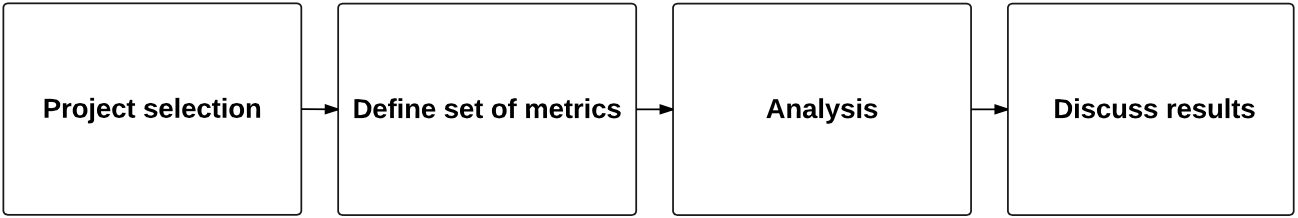
\includegraphics[width=1\textwidth]{figures/approach_overview}
 \end{figure*}
After selecting projects we have to find an automatic way to have all versions downloaded, and ready for analysis. Instead of downloading each version separately, we devise a viable and more efficient technique. We cloned latest release containing \textit{\.git} folder in it. Then we write a script to checkout each tag based on the tags that git gives us by running \textit{git tag}.
\par
Each version of each application has been analyzed with a powerful source code analyzer tool named SonarQube to extract metrics relevant to evolution of software. We also used this tool catch anti-patterns developers do in JavaScript and categorize them based on their severity.
To have all these data get analyzed in SonarQube we had to deal few unexpected behavior. For example SonarQube does not consider release dates as the real release date. It just take out the date of the analysis that it fires to analyze a source. In this scenario we have 1065 releases with the release date of the day we ran analysis. So we fixed the issue to have proper release dates.

\par After analyzing every tag in SonarQube we extract our chosen metrics that we found them proper for studying evolution of JavaScript projects. Metrics such as McCabe cyclomatic complexity,  comment line density, duplicated lines and blocks, number of directories and statements and etc. Table  \ref{tab:metrics_definition} defines sets of metrics that we used in our analysis.


\begin{table*}[!hbt]
	\begin{center}
		\caption{Release details from each analyzed project}
		\label{tab:metrics_definition}
		\begin{tabular}{c| l l }
			\toprule
			\textbf{Metric} & \textbf{Definition} \\ \midrule
			Lines of Code & The number of uncommented lines of code    \\
			Complexity      & McCabe complexity    \\
			Complexity/function & Average complexity by function. \\
			Complexity/file & Average complexity by file \\
			Comment lines  & Number of lines containing either comment or commented-out code. \\
			Comment Lines (\%)   & Density of comment lines = Comment lines / (Lines of code + Comment lines) * 100    \\
			Duplicated lines (\%)     & Density of duplication = Duplicated lines / Lines * 100    \\
			Duplicated blocks   & Number of duplicated blocks of lines    \\
			Directories   & Number of directories    \\
			Functions            & Number of functions    \\
			Statements      & Number of functions   \\
			Issues    & Number of issues with severity of blocker, critical, major and minor   \\
		SQALE Rating   & ?????????    \\
			Technical debt    & Number of days it takes to fix issues with respect to their severity    \\
			Technical debt ratio   & Division of SQALE Index by the estimation effort to re-develop your application from scratch.    \\
		\end{tabular}
	\end{center}
\end{table*}



\subsection{Project Selection}

In selecting projects for our study, we used several criteria. First, we selected projects that are popular between developers and with a large number of users, since we want to analyze their evolution, it is important that they are active projects. Second, we used projects that have their source code and issuer tracker both hosted in GitHub. This makes easier to collect information about collaboration and measure popularity of the projects. Besides, GitHub provides us an API to extract data from their repositories that will collaborate with the evolution analysis that we will run. Third we consider at this point projects with similar sizes. We will enhance this criteria with size and application domain in our final report so we can be more assertive when searching for insights about the evolution of the projects. However it is not possible to have the real-world projects with the same size in these two different languages. So we will apply some normalization approach, to make sure we are able to compare these two different worlds.

Regarding the lifespan of the analyzed projects we considered 5 previous full releases, regardless of the time that it took to be released. We consider a full release accordingly to the analyzed project. These releases are the ones with major changes in design and addition of new features as well, because of that we considered them as good candidates to conduct our study.  

As mentioned, before we ran our analysis in 10 open source projects, five of them were written in JavaScript and namely they are as following: NPM a package manager for JavaScript, Node MySQL a pure node.js JavaScript Client implementing the MySql protocol, Esprima a high performance and standard-compliant JavaScript parser, Grunt a JavaScript task runner and Node Redis a Redis client for node. Table \ref{tab:java_script_proj_details} presents hight level data of these projects.

In the same way the five Java projects analyzed were ElasticSearch is aa distributed, RESTful search engine, Gauva is the Google Core Libraries for Java 6+, JodaTime is widely used as replacement for the Java date and time classes, Jsoup is a Jason library for Java and finally JUnit is an unit test framework for Java. Their data are presented in Table \ref{tab:java_proj_details}     

\begin{table*}[!tbh]
	\begin{center}
		\caption{JavaScript Project Details }
		\label{tab:java_script_proj_details}
		\begin{tabular}{l| c c c c c}
			\toprule
			\textbf{Project} & \textbf{\# of JS files in latest release} & \textbf{Number of Directories} & \textbf{LOC\footnote{Lines of code}} & \textbf{Number of Functions} & \textbf{Number of Statements} \\ 
			\midrule
			NPM              & 165                                       & 32                             & 9,075                                & 1,217                        & 5,329                         \\
			Node MySQL       & 140                                       & 11                             & 4,720                                & 667                          & 3,317                         \\
			Esprima          & 34                                        & 6                              & 83,385                               & 4,862                        & 29,002                        \\
			Grunt            & 31                                        & 9                              & 2,361                                & 251                          & 1,245                         \\
			Node Redis       & 18                                        & 6                              & 2,529                                & 457                          & 2,537                         \\ 
			\bottomrule
		\end{tabular}
	\end{center}
\end{table*}

\begin{table*}[!tbh]
	\begin{center}
		\caption{Java Project Details }
		\label{tab:java_proj_details}
		\begin{tabular}{l| c c c c c c}
			\toprule
			\textbf{Project} & \textbf{\# of JS files in latest release} & \textbf{Number of Directories} & \textbf{LOC} & \textbf{Number of Functions} & \textbf{Classes} & \textbf{Number of Statements} \\ 
			\midrule
			ElasticSearch    & 4,050                                     & 831                            & 424,007                              & 35,762                       & 5,967            & 198,944                       \\
			Gauva            & 799                                       & 28                             & 90,401                               & 11,769                       & 1,644            & 32,698                        \\
			JodaTime         & 327                                       & 15                             & 84,855                               & 9,560                        & 473              & 50,609                        \\
			Jsoup            & 80                                        & 14                             & 13,672                               & 1,487                        & 154              & 7,980                         \\
			JUnit            & 392                                       & 73                             & 26,079                               & 3,479                        & 1,063            & 7,972                         \\ 
			\bottomrule
		\end{tabular}
	\end{center}
\end{table*}

%\begin{table*}\label{eval_table}\centering
%	\caption{Proposed experiment projects with preliminary results of most recent version of release in our dataset}
%	\begin{threeparttable}
%		\scalebox{0.7}{
%			\begin{tabular}{llccccc}
%				\toprule
%				Project & Description &  {\# of JS files in latest release} & Number of Directories & LOC \footnote{Lines of code}& Number of Functions & Number of Statements  \\
%				\addlinespace
%				\midrule
%				NPM & Package manager for JavaScript & 165 & 32 & 9,075 & 1,217 & 5,329  \\
%				\addlinespace
%				\midrule
%				Node MySQL & A pure node.js JavaScript Client implementing the MySql protocol.  & 140 & 11& 4,720 & 667 & 3,317 \\			
%				\addlinespace 	
%				\midrule
%				Esprima & A high performance, standard-compliant JavaScript parser written in JavaScript  & 34 & 6 & 83,385 & 4,862 & 29,002  \\
%				\addlinespace		
%				\midrule
%				Grunt & The JavaScript Task Runner & 31 & 9 & 2,361 & 251 & 1,245 \\
%				\addlinespace
%				\midrule
%				Node Redis & Redis client for node & 18 & 6 & 2,529 &  457 & 2,537   \\	
%				\addlinespace 
%				
%			\end{tabular}
%		}
%	\end{threeparttable}
%\end{table*}
%
%\begin{table*}\label{tab:eval_java}\centering
%	\caption{Proposed experiment projects with preliminary results of most recent version of release in our dataset}
%	\begin{threeparttable}
%		\scalebox{0.7}{
%			\begin{tabular}{llccccccc}
%				\toprule
%				Project & Description & {\# of java files in latest release} & Number of Directories & LOC & Number of Functions & classes & Number of Statements \\
%				\addlinespace
%				\midrule
%				ElasticSearch & Open Source, Distributed, RESTful Search Engine 
%				& 4,050 & 831 & 424,007 & 35,762 & 5,967 & 198,944 \\
%				\addlinespace
%				\midrule
%				Gauva & Google Core Libraries for Java 6+ & 799 & 28 & 90,401 & 11,769 & 1,644 & 32,698\\    
%				\addlinespace 
%				\midrule
%				JodaTime & Joda-Time is the widely used replacement for the Java date and time classes. & 327 & 15 & 84,855 & 9,560 & 473 & 50,609 \\
%				\addlinespace    
%				\midrule
%				Jsoup & Jason library for java & 80 & 14 & 13,672 & 1,487 & 154 & 7,980 \\
%				\addlinespace
%				\midrule
%				JUnit & Unit test framework for java & 392 & 73 & 26,079 & 3,479 & 1,063 & 7,972  \\   	
%				\addlinespace 
%			\end{tabular}
%		}
%	\end{threeparttable}
%\end{table*}

\subsection{Define set of metrics}

Lehman suggests using the number of “modules” as the best way to measure the size of a large software system \cite{Lehman1997METRICS}. However, we decided to use the number of uncommented lines of code (“uncommented LOC”) like the way Godfrey et al \cite{Godfrey2000ICMS} did the evolution study on Linux Kernel. On the other hand we measure the comment lines and the ratio of comments to lines of codes, and based on that we can infer how much developers tend to put comments within their codes. We have to consider hidden corners that can mislead results, for example descriptive comments are totally different to the lines of codes that got commented because of refactoring or changes which consider as light-weight code smells within the code.

We want to measure various aspects of the growth of these applications by having metrics such as number of files, lines of code, number of functions and statements. We also measure amount of duplications known as clones in terms of lines of codes, blocks and files. We would measure the cyclomatic complexity over time which the metric is calculated as following. Whenever the control flow of a function splits, the complexity counter gets incremented by one. Each function has a minimum complexity of 1. The control flow can split by conditional statements like if/else, switch case and so on. This metric is also known as also known as McCabe metric
We use the term “source file” to mean any file whose name ends with “.js” and also we removed folders containing external libraries which is usually located at \textit{lib} or \textit{node\_modules}. 

We also measure the amount of object oriented principles that JavaScript developers use in their day to day software development. We think if we quantify the amount of reusable parts (i.e classes) in these projects, there are some valuable reasons laid down related to evolution behind these techniques. Consequently we use a project, known as JSDeodorant to find class declarations and places developers instantiate objects.
In the rest of this section we describe how developers create objects in JavaScript and how they mimic object oriented class definitions without having direct language support in the specification of language.

\noindent\textbf{Creation Types:} Here, we explain different types of object creation no matter if they are built-in type or user-defined. 
%\subsubsection{Creation Types}

\medskip
\noindent\subsubsection{Array Literal Expression}
%\duptype{\textbf{Type I}: \textit{Array Literal Expression}.}

it creates a string array consisting of three creations possible in JavaScript elements and is assigned to variable “cars” using a binary operator (with two operand and equal operator). 
\medskip
\begin{lstlisting}[caption={Array literal expression},label={lst:array_literal},language=JavaScript]
var cars = ['Saab', 'Volvo', 'BMW'];
\end{lstlisting}
A JavaScript array is initialized with the given elements, except in the case where a single argument is passed to the Array constructor and that argument is a number. Note that this special case only applies to JavaScript arrays created with the Array constructor, not array literals created with the bracket syntax.
\\
%\break
%\duptype{\textbf{Type II}: \textit{Array Creation using \textbf{new} keyword}.}
\noindent\subsubsection{Array Creation using \textbf{new} keyword}

The Array constructor function with using the “New” keyword creates an array of three elements and then assigned the created object to variable “planes” using binary operator. Using the more verbose method: \textit{new Array()} instead of array literal expression does have one extra option in the parameters: if you pass a number to the constructor, you will get an array of that length. 

\medskip
\begin{lstlisting}[caption={Array constructor},label={lst:array_constructor},language=JavaScript]
var planes= new Array('Boeing', 'Airbus', 'Bombar- dier');
\end{lstlisting}

\noindent\subsubsection{Object Literal Expression}

%\duptype{\textbf{Type III}: \textit{Object Literal Expression}.}

The created object is basically singletons with variables/methods that are all public. An object literal is a comma-separated list of name-value pairs wrapped in curly braces. Object literals encapsulate data, enclosing it in a tidy package. This minimizes the use of global variables which can cause problems when combining code. If any of the syntax rules are broken, such as a missing comma or colon or curly brace, a JavaScript error will be triggered. No need to invoke constructors directly or maintain the correct order of arguments passed to functions.
\begin{lstlisting}[caption={Object literal expression},label={lst:object_literal_expression},language=JavaScript] 
var myObj = {
	myMethod: function(params) {
		// ...do something
	}
};
\end{lstlisting}

\noindent\subsubsection{Function Constructor}
%\duptype{\textbf{Type IV}: \textit{Function Constructor}.}

Listing \ref{lst:function_constructor}, shows the function constructor, there we define a function that should start with an uppercase letter by convention (to inform call sites use this function with “new” keyword). The Function constructor creates a new Function object and in JavaScript every function is actually a Function object.

Parameters are Names to be used by the function as formal parameter names. Each must be a string that corresponds to a valid JavaScript identifier or a list of such strings separated with a comma. Functions created with the Function constructor do not create closures to their creation contexts; they always are created in the global scope.

When running them, they will only be able to access their own local variables and global ones, not the ones from the scope in which the Function constructor was called.

\begin{lstlisting}[caption={Function constructor},label={lst:function_constructor},language=JavaScript] 
function Employee(name){
	this.name = name;
	this.getName = function(){
		return this.name;
	};	
};
var emp = new Employee ('John');
\end{lstlisting}
	
\section{Case Study results}
\label{sec:results}

\begin{table*}[!hbt]
	\begin{center}
		\caption{Release details from each analyzed project}
		\label{tab:evolution_overview}
		\begin{tabular}{l l| c c c c c c c}
			\toprule
			\textbf{Project}  & \textbf{Release} & \textbf{LOC} & \textbf{Commented lines} & \textbf{Directories} & \textbf{Functions} & \textbf{Statements} & \textbf{Complexity} & \textbf{\# Developers}\\ \midrule              
			\multirow{2}*{Coffeescript}& First  0.6.1                   &           4693 &           836 &           3 &       915 &       5916 &       2958\\
			& Last   1.9.0                   &           7723 &           124 &           6 &      1262 &       6687 &       5251\\ \midrule
			\multirow{2}*{Less.js     }& First  v1.0                    &           1269 &           279 &           6 &       179 &        818 &        634\\
			& Last   v2.3.1                  &          18585 &          2085 &          18 &      2605 &      13609 &       9414\\ \midrule
			\multirow{2}*{Npm         }& First  v0.0.7                  &           1979 &           259 &           3 &       238 &       1234 &        780\\
			& Last   v2.7.4                  &          19837 &          1060 &          34 &      2469 &      12004 &       5918\\ \midrule
			\multirow{2}*{Mongoose    }& First  0.0.1                   &            554 &            12 &           6 &       100 &        373 &        217\\
			& Last   4.0.1                   &          41844 &          5710 &          12 &      5749 &      27722 &       9373\\ \midrule
			\multirow{2}*{Underscore  }& First  1.0.3                   &           1127 &           154 &           2 &       376 &       1317 &        738\\
			& Last   1.8.0                   &           3918 &           385 &           2 &       849 &       3719 &       1650\\ \midrule
			\multirow{2}*{Node-mysql  }& First  v0.1.0                  &           2431 &            55 &           4 &       203 &       1876 &        435\\
			& Last   v2.6.0                  &          10701 &           430 &          16 &      1046 &       8044 &       2010\\ \midrule
			\multirow{2}*{Q           }& First  v0.1.0                  &            188 &            95 &           1 &        35 &        113 &         64\\
			& Last   v1.1.2                  &           6670 &          1149 &           6 &      1396 &       4118 &       2182\\ \midrule
			\multirow{2}*{Request     }& First  v1.2.0                  &            312 &            12 &           2 &        24 &        214 &        112\\
			& Last   v2.54.0                 &           7839 &           333 &           5 &       958 &       4086 &       1713\\ \midrule
			\multirow{2}*{Ember.js    }& First  sc-v2.0.beta.1          &          28582 &         10006 &          67 &      3879 &      21402 &       9743\\
			& Last   v1.11.0-beta.5          &          65548 &         14698 &         115 &      9323 &      38894 &      13878\\ \midrule
			\multirow{2}*{Source-map  }& First  0.1.0                   &           1214 &           855 &           5 &       124 &        669 &        271\\
			& Last   0.4.1                   &           4485 &           791 &           7 &       322 &       2362 &        757\\ \midrule
			\multirow{2}*{Bootstrap   }& First  v1.3.0                  &            886 &           105 &           2 &       130 &        510 &        261\\
			& Last   v3.3.2                  &           6834 &           358 &           5 &       980 &       4532 &       2337\\ \midrule
			\multirow{2}*{Mocha       }& First  0.0.1-alpha1            &           1185 &           284 &           6 &       226 &        703 &        309\\
			& Last   2.2.0                   &           9931 &          2229 &          21 &      1750 &       6586 &       3197\\ \midrule
			\multirow{2}*{Brackets    }& First  sprint-1                &           6271 &          1198 &          14 &      1305 &       4234 &       2183\\
			& Last   release-1.2-prerelease1 &         266801 &         63923 &         179 &     27845 &     148274 &      82848\\ \midrule
			\multirow{2}*{Bower       }& First  v0.1.1                  &           1149 &           117 &           9 &       212 &        856 &        423\\
			& Last   v1.4.0                  &          15802 &          1439 &          17 &      2454 &       8641 &       3646\\ \midrule
			\multirow{2}*{Grunt       }& First  v0.4.0                  &           3972 &           682 &          11 &       492 &       2482 &        886\\
			& Last   v0.4.4                  &           4010 &           663 &          12 &       498 &       2447 &        874\\ \bottomrule
		\end{tabular}
	\end{center}
\end{table*}

\par
To summarize the distance between first and last release of each project we use different metrics based on Table \ref{tab:metrics_definition} metrics and list them in Table \ref{tab:evolution_overview}. 
As we can see Brackets first release contains 6271 lines of code but it ends up with 266801 lines of code in the last release. Bracket's last release is the most biggest evolved project with in four years of its existence. It started with 14 directories which in the last release it contains 179 directories. Brackets has 60 releases during its lifetime with 15871 commits. On the other hand NPM with 298 releases is the project with most releases in our dataset. It starts with 1979 lines of code where the last release exceeds to 19837 lines of code with 2231 functions added since the first release. To better understand the detail of evolution we depict the growth of LOC, directories, functions, statements and complexity.  

% release_density 

% function_density Figure Release density in NPM and Grunt where x is year and y is number of releases


\par
In terms of adopting object oriented practices we can infer that Sourcemap is the project that has function density of 10.2 with the lowest rank and Bootstrap as the most dense project that adopt re-usability by having 40.6 function density in lines of codes.
The way developers define function can be varied in JavaScript code. Figure \ref{fig:function_density} indicates evolution of our five selected projects. Short after the project initiated, Bootstrap rocketed to have more than 300\%. The function density calculates based on the following formula: 
\begin{center}
$\frac{Number\space of\space Functions}{Lines \space of\space code}*100$
\end{center}


\par For number of developers we tried to gather data based on email of authors that commit code, however we found out that authors can have multiple emails register to one login id. As a result we tried to count the number of developers based on the Github usernames. 

 \begin{figure}[thb!]
 	\caption{Function density evolution}
 	\label{fig:function_density}
 	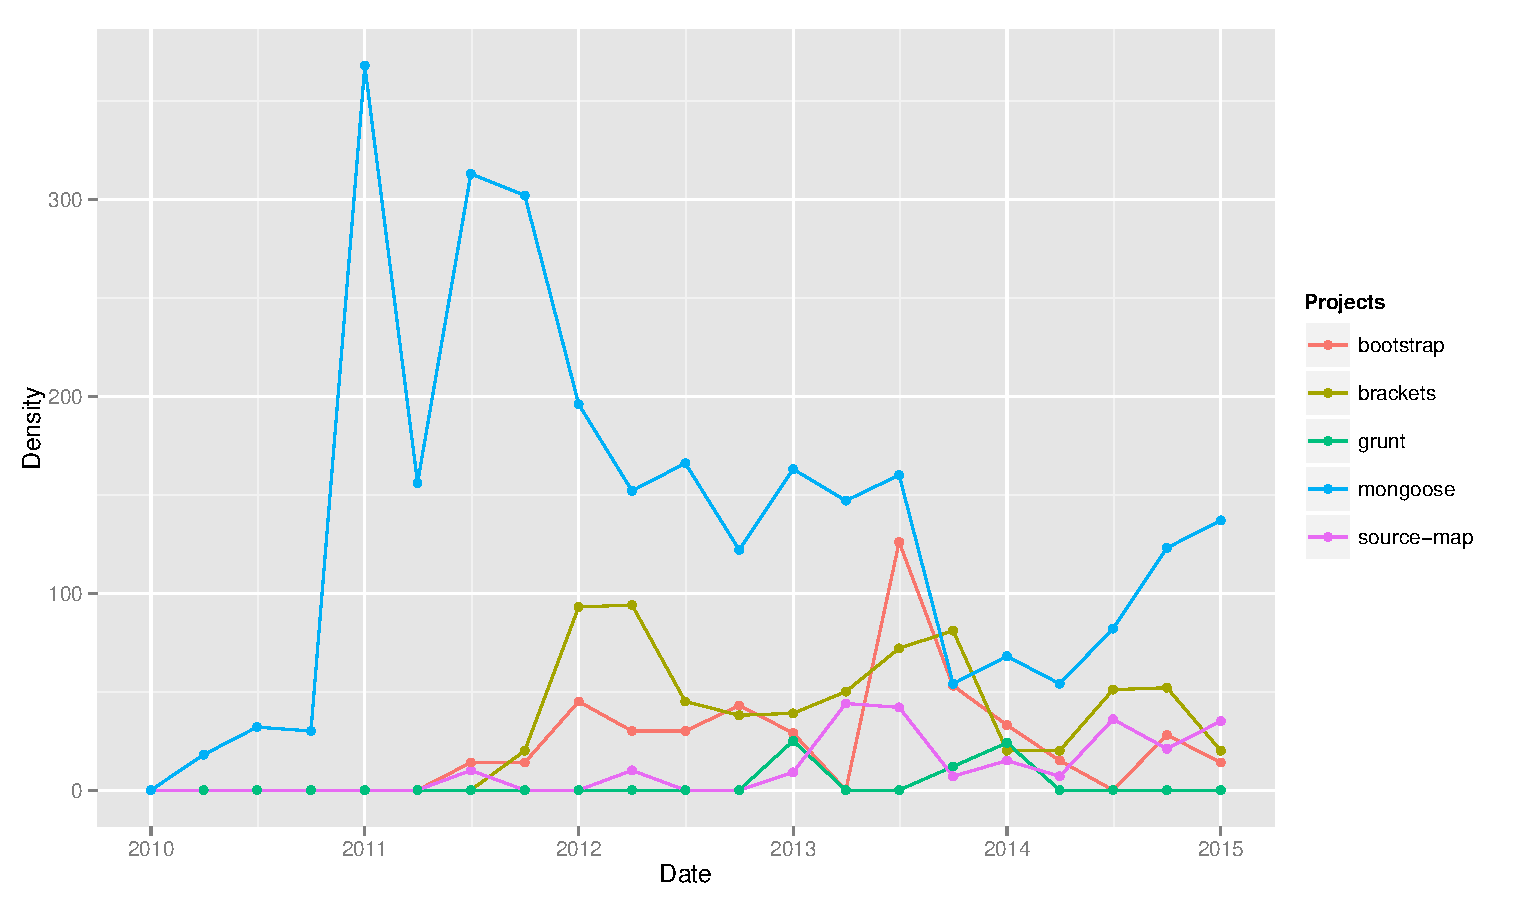
\includegraphics[width=90mm,scale=0.5]{figures/function_density}
 \end{figure}


\par
Having comments as one of the artifacts that can improve the readability of source code we examined it as metric of evolution.
Brackets has the most comment lines with having 63923 comment lines followed by Ember.js with 14698 comment lines. The least documented project is CoffeeScript with having only 124 lines of documentation. What makes the resuls interesting, is the fact that CoffeeScript starts with 836 lines of comments in the first release but in the last release we have only 124 lines of code. CoffeeScript and Grunt are the only projects that adapt this pattern, while all the other projects show growing trend in number of comments during evolution.  


\par
% developers_release

\section{Threats to validity}
\label{sec:threats}
\par
We found one project was migrated from SVN before the first commit in git. Github keeps track of tags that were imported from another source control but based on unknown reasons it does not import commits. So we faced with a scenario that we tag with date before first commit initiated on Github. 


\par
Moreover, all of the projects that we select are either server side codes or they are client side libraries for enhancement of development in client side web applications. But we did not take it into account to have JavaScript codes that are part of the web application. The results from client site codes which are not part of client libraries can reflect different behavior than what we observe on our selected dataset.


\section{Related Work}
\label{sec:related_work}
Kyriakakis \emph{et al.} \cite{Kyriakakis2014ICMSE} Analyzed the evolution of PHP projects over time. Their work contributes to the evolution scenario because script languages as PHP are often labeled as inappropriate for big projects, under the claim that these languages are not maintainable. During their experiment they analyzed the evolution of five open source projects with a long development history. They analyzed the amount of unused code, the removal of functions, the use of libraries, the stability of the interfaces, the migration to object-orientation and the evolution of complexity. Based on their results they concluded that these projects are submitted to organized changes and perfective maintenance does stills takes place in the projects. They also find that all the projects are gradually migrating to object-orientation fact that indicates planed maintenance as this feature was added in the language after the start of the development of all projects. 

Similarly to this work we pretend to understand how the JavaScript language evolves over time, collaborating with the script languages evolution landscape. In addition to that, we search for possible applications of lessons learned analyzing the evolution of static languages as Java. Finding similar evolution patterns between script and static languages will lead us to best practices that can be applied in both contexts. 

Godfrey \emph{et al.} \cite{Godfrey2000ICMS} analyzed how large open source projects would evolve over time. Until their research, most work in software evolution was related with ``in home'' solutions. They collected and analyzed 6 years of development data from Linux kernel a large open source project with over two million of lines of code in the latest version analyzed at the time. They measured the length of the each full distribution, the lines of code (considering commented and blanks lines and then ignoring them as well), the number of global functions, variables and macros. They found that Linux kernel growth has been super-linear despite the fact of its large size, the collaboration of several volunteers developers that are scattered around the world and that previous research in the area had found that growth of large software systems tends to slow down as the system becomes larger. They also found several important facts particular to the Linux Kernel system as although the source tree for Linux is rather large more than half of the code belongs to devices drivers. 

Xie \emph{et al.} \cite{Xie2009ICSM} also analyses the evolution of open source projects. As there are controversial statements about the evolution of open source projects they decided to conduct their work analyzing first, how Lehman's eight laws of software evolution \cite{Lehman1997METRICS} can be applied in open source projects. Second, they analyze the growth rate of the development and maintenance branches and the distribution of software changes. To conduct this research, they collected historical development data from 7 open source projects, a total of 653 official releases and over 69 years of cumulative program evolution. They found that the first four of the Lehman's laws - Continuing Change, Increasing Complexity, Self Regulation and Continuing Growth - are still applicable in open source software, whereas the other four - Conservation of Organizational Stability, Conservation of Familiarity, Declining Quality and Feedback System - were not possible to validate because of inconclusive results. In addition to that they found that the development branch and the maintenance branch evolves in parallel and that a high percentage of changes are concentrated to a small percentage of code.    

Like these previous works we analyze the evolution of open source projects, but in particular we focus our analyzes in several small to mid-sized open sources projects written in two different languages, one dynamic (JavaScript) and the other one static (Java). We conduct an empirical study to analyze two main factors, first how JavaScript projects evolves over time and second, what are the lessons from static languages that can be applied as a good practice in JavaScript.
 

\section{Future Work}
\label{sec:future}
Our approach followed an automatic mechanism to extract, refine and analyze source codes without human intervention. By utilizing this approach we are able to have a big data set helping us to achieve more precise result. Certainly we want to have equal number of Java projects to be able comparing evolution of these two different language. SonarQube is capable of measuring metrics regardless of target language. That study would certainly reveal hidden corners that we did not catch by studying only JavaScript projects and if the outcome shows similarities, making decision for stakeholders, project owners and developers would be easier to have best practices from Java which established for more than a decade in an enterprise level applications.
JavaScript lacks standard language specification for defining classes. Classes are used to achieve re-usability in JavaScript. We developed a tool for finding these classes using static analysis. For another study we extract object oriented metrics from well-known JavaScript such as McCabe cyclomatic complexity, coupling between objects \cite{Briand-Coupling} and cohesion\cite{Briand-Cohesion}. These metrics can help us to better understand JavaScript projects and also we can compare these metrics with values extracted from Java projects correspondingly. 
We plan to extensively study differences and similarities between Java and JavaScript project to gain deeper insight into these two different world. To achieve our goal we have been considering every corner cases we would face in our study like lacking of explicit class definition in JavaScript and different style of defining namespaces in JavaScript. Namespaces are the only way JavaScript developers rely to achieve higher degree of granularity.

\section{Conclusion}
\label{sec:conclusion}
We conduct an empirical study in the evolution of JavaScript projects. We analyzed 15 open source projects from different domains of application. In general each one of the projects has more than 5 years of development history allowing us to explore over 57 years of software evolution.

First we analyze how JavaScript projects grows over time. We measured all the projects by the following attributes: lines of code, number of commented lines, number of directories, number of functions, statements and complexity. We found that all the projects increased with very pace , and some times with huge leaps in the number of lines of code from one version to another. This is due mostly to the dynamic environment and the community that surrounds JavaScript projects (e.g., A popular project will draw many developers to join the development) in addition to the customization of open source libraries that becomes part of the project own source code. 

We found that developers are worried about evolving the project in a maintainable manner as we can see an increase in the commented lines and in the number of directories as the time goes by. We infer that the growth of directories is a signal of modularization in JavaScript projects, as the language does not support directly the creation of namespaces. Other than that, the grow of commented lines is a signal of code documentation in JavaScript. However, more research is needed to collect more evidence of these behavior.

Second, we analyze the average time to ship new releases and the changes in the public APIs. We found that versions tend to be released fast in most of the projects. The most active project was NPM with an average of 5.13 releases per month, and the lowest average belongs to Grunt with 0.41 releases a month. Regarding the changes in the API, we found that the analyzed projects tend to have changes in their APIs until they reach a maturity point and become stable during several releases. The time to reach maturity varies from project to project.

Third, we found that the JavaScript community has many independent contributors beside the core-developers, although this characteristic varies with the size and domain of the project. In terms of time to fix a bug we found that for 86\% of the analyzed projects it takes less than 60 days to fix a bug. The fastest project to fix a bug was Bootstrap with an average of 11 days and the slowest is project Less with an average of 113 days.  

Fourth, we analyzed how common are the anti-patterns in JavaScript software and how severe they are. We found that anti-patterns appears in JavaScript projects with frequency. However, they are not the most severe kind of faults. The concentration of these anti-patterns are mostly in two categories, major and minor. The tendency of these anti-patterns over time is increasing, but we found an exception in Ember.js where this trend shows decreasing.   

\bibliographystyle{IEEEtran}
\bibliography{design_td}

\end{document}